% \documentclass{beamer}
\documentclass[hyperref={unicode}]{beamer}

\usepackage{amsmath}
\usepackage{datetime2}
\usepackage[numbers]{natbib}
\usepackage{graphicx}

\DTMnewdatestyle{mydateformat}{%
  \renewcommand{\DTMdisplaydate}[4]{%
    \number##1\ % year
    \DTMenglishmonthname{##2}\ % Month
    \number##3% day
  }%
  \renewcommand{\DTMDisplaydate}{\DTMdisplaydate}%
}
\DTMsetdatestyle{mydateformat}

\bibliographystyle{amsalpha}

\usetheme{Darmstadt}
\beamertemplatenavigationsymbolsempty

\title{Persistent Homology}
\subtitle{Computations and Applications}
\author{Stephen Ermshar}
\institute{Walla Walla University}
\date{\DTMDisplaydate{2020}{3}{13}{}}


\title{Persistent Homology}
\subtitle{Computations and Applications}
\author{Stephen Ermshar}
\institute{Walla Walla University}
\date{\DTMDisplaydate{2020}{3}{13}{}}

\begin{document}




\begin{frame}
    \titlepage
\end{frame}

\begin{frame}{Outline}
	\tableofcontents
\end{frame}

\section[Homology]{Homology}
\subsection{Simplicial Homology}
\begin{frame}
	\begin{figure}
		\tikzset{every picture/.style={line width=0.75pt}} %set default line width to 0.75pt

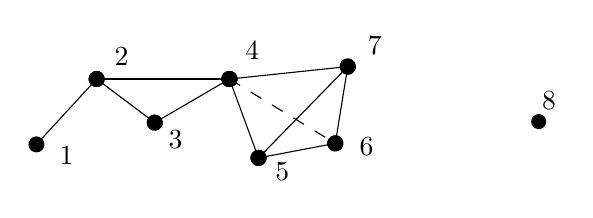
\begin{tikzpicture}[x=0.75pt,y=0.75pt,yscale=-1,xscale=1]
%uncomment if require: \path (0,95); %set diagram left start at 0, and has height of 95

%Straight Lines [id:da20686486428426965]
\draw    (13,61) -- (42,29.5) ;
\draw [shift={(42,29.5)}, rotate = 312.63] [color={rgb, 255:red, 0; green, 0; blue, 0 }  ][fill={rgb, 255:red, 0; green, 0; blue, 0 }  ][line width=0.75]      (0, 0) circle [x radius= 3.35, y radius= 3.35]   ;
\draw [shift={(13,61)}, rotate = 312.63] [color={rgb, 255:red, 0; green, 0; blue, 0 }  ][fill={rgb, 255:red, 0; green, 0; blue, 0 }  ][line width=0.75]      (0, 0) circle [x radius= 3.35, y radius= 3.35]   ;
%Straight Lines [id:da9899744043809231]
\draw    (42,29.5) -- (106,29.5) ;
\draw [shift={(106,29.5)}, rotate = 0] [color={rgb, 255:red, 0; green, 0; blue, 0 }  ][fill={rgb, 255:red, 0; green, 0; blue, 0 }  ][line width=0.75]      (0, 0) circle [x radius= 3.35, y radius= 3.35]   ;
\draw [shift={(42,29.5)}, rotate = 0] [color={rgb, 255:red, 0; green, 0; blue, 0 }  ][fill={rgb, 255:red, 0; green, 0; blue, 0 }  ][line width=0.75]      (0, 0) circle [x radius= 3.35, y radius= 3.35]   ;
%Straight Lines [id:da4483952202454973]
\draw    (42,29.5) -- (70,50.5) ;
\draw [shift={(70,50.5)}, rotate = 36.87] [color={rgb, 255:red, 0; green, 0; blue, 0 }  ][fill={rgb, 255:red, 0; green, 0; blue, 0 }  ][line width=0.75]      (0, 0) circle [x radius= 3.35, y radius= 3.35]   ;
\draw [shift={(42,29.5)}, rotate = 36.87] [color={rgb, 255:red, 0; green, 0; blue, 0 }  ][fill={rgb, 255:red, 0; green, 0; blue, 0 }  ][line width=0.75]      (0, 0) circle [x radius= 3.35, y radius= 3.35]   ;
%Straight Lines [id:da013663715151336797]
\draw    (70,50.5) -- (106,29.5) ;
\draw [shift={(106,29.5)}, rotate = 329.74] [color={rgb, 255:red, 0; green, 0; blue, 0 }  ][fill={rgb, 255:red, 0; green, 0; blue, 0 }  ][line width=0.75]      (0, 0) circle [x radius= 3.35, y radius= 3.35]   ;
\draw [shift={(70,50.5)}, rotate = 329.74] [color={rgb, 255:red, 0; green, 0; blue, 0 }  ][fill={rgb, 255:red, 0; green, 0; blue, 0 }  ][line width=0.75]      (0, 0) circle [x radius= 3.35, y radius= 3.35]   ;
%Straight Lines [id:da6445202628566384]
\draw    (106,29.5) -- (163,23.5) ;
\draw [shift={(163,23.5)}, rotate = 353.99] [color={rgb, 255:red, 0; green, 0; blue, 0 }  ][fill={rgb, 255:red, 0; green, 0; blue, 0 }  ][line width=0.75]      (0, 0) circle [x radius= 3.35, y radius= 3.35]   ;
\draw [shift={(106,29.5)}, rotate = 353.99] [color={rgb, 255:red, 0; green, 0; blue, 0 }  ][fill={rgb, 255:red, 0; green, 0; blue, 0 }  ][line width=0.75]      (0, 0) circle [x radius= 3.35, y radius= 3.35]   ;
%Straight Lines [id:da3743946516627876]
\draw    (106,29.5) -- (120,67.5) ;
\draw [shift={(120,67.5)}, rotate = 69.78] [color={rgb, 255:red, 0; green, 0; blue, 0 }  ][fill={rgb, 255:red, 0; green, 0; blue, 0 }  ][line width=0.75]      (0, 0) circle [x radius= 3.35, y radius= 3.35]   ;
\draw [shift={(106,29.5)}, rotate = 69.78] [color={rgb, 255:red, 0; green, 0; blue, 0 }  ][fill={rgb, 255:red, 0; green, 0; blue, 0 }  ][line width=0.75]      (0, 0) circle [x radius= 3.35, y radius= 3.35]   ;
%Straight Lines [id:da2401873796980163]
\draw    (120,67.5) -- (163,23.5) ;
\draw [shift={(163,23.5)}, rotate = 314.34] [color={rgb, 255:red, 0; green, 0; blue, 0 }  ][fill={rgb, 255:red, 0; green, 0; blue, 0 }  ][line width=0.75]      (0, 0) circle [x radius= 3.35, y radius= 3.35]   ;
\draw [shift={(120,67.5)}, rotate = 314.34] [color={rgb, 255:red, 0; green, 0; blue, 0 }  ][fill={rgb, 255:red, 0; green, 0; blue, 0 }  ][line width=0.75]      (0, 0) circle [x radius= 3.35, y radius= 3.35]   ;
%Straight Lines [id:da08347218855288774]
\draw  [dash pattern={on 4.5pt off 4.5pt}]  (106,29.5) -- (157,60.5) ;
\draw [shift={(157,60.5)}, rotate = 31.29] [color={rgb, 255:red, 0; green, 0; blue, 0 }  ][fill={rgb, 255:red, 0; green, 0; blue, 0 }  ][line width=0.75]      (0, 0) circle [x radius= 3.35, y radius= 3.35]   ;
\draw [shift={(106,29.5)}, rotate = 31.29] [color={rgb, 255:red, 0; green, 0; blue, 0 }  ][fill={rgb, 255:red, 0; green, 0; blue, 0 }  ][line width=0.75]      (0, 0) circle [x radius= 3.35, y radius= 3.35]   ;
%Straight Lines [id:da34695654406224863]
\draw    (120,67.5) -- (157,60.5) ;
\draw [shift={(157,60.5)}, rotate = 349.29] [color={rgb, 255:red, 0; green, 0; blue, 0 }  ][fill={rgb, 255:red, 0; green, 0; blue, 0 }  ][line width=0.75]      (0, 0) circle [x radius= 3.35, y radius= 3.35]   ;
\draw [shift={(120,67.5)}, rotate = 349.29] [color={rgb, 255:red, 0; green, 0; blue, 0 }  ][fill={rgb, 255:red, 0; green, 0; blue, 0 }  ][line width=0.75]      (0, 0) circle [x radius= 3.35, y radius= 3.35]   ;
%Straight Lines [id:da5097015872445443]
\draw    (163,23.5) -- (157,60.5) ;
\draw [shift={(157,60.5)}, rotate = 99.21] [color={rgb, 255:red, 0; green, 0; blue, 0 }  ][fill={rgb, 255:red, 0; green, 0; blue, 0 }  ][line width=0.75]      (0, 0) circle [x radius= 3.35, y radius= 3.35]   ;
\draw [shift={(163,23.5)}, rotate = 99.21] [color={rgb, 255:red, 0; green, 0; blue, 0 }  ][fill={rgb, 255:red, 0; green, 0; blue, 0 }  ][line width=0.75]      (0, 0) circle [x radius= 3.35, y radius= 3.35]   ;


% Text Node
\draw (27.5,66.5) node    {$1$};
% Text Node
\draw (54,18.5) node    {$2$};
% Text Node
\draw (80,58.5) node    {$3$};
% Text Node
\draw (117,16) node    {$4$};
% Text Node
\draw (131.5,74) node    {$5$};
% Text Node
\draw (172,62) node    {$6$};
% Text Node
\draw (176,13.5) node    {$7$};
% Text Node
\draw[fill={rgb, 255:red, 0; green, 0; blue, 0 }] (255, 50) circle [x radius= 3.35, y radius= 3.35]    (260,40) node    {$8$};



\end{tikzpicture}

		\caption{Example Simplicial Complex with one hole and one void.}
	\end{figure}
\end{frame}
\subsection{Computations}
\begin{frame}
\end{frame}


\section[Persistence]{Persistent Homology}
\subsection{\v{C}ech, Rips, and Witness Complexes}
\begin{frame}
\end{frame}

\section{Applications}
\subsection{Visualization and Compression}
\begin{frame}
\end{frame}

\section{Bibliography}
\begin{frame}{Bibliography}
	\nocite{wagner}
	\nocite{hatcher}
	\nocite{singh}
	% https://tex.stackexchange.com/a/22654
	\begingroup
	\renewcommand{\section}[2]{}%
	\bibliography{../math496-7-zotero.bib}
	\endgroup
\end{frame}




\end{document}
